% !TEX spellcheck = en_US
% Wind field
%=================================================================================
To test the turbine model in Simulink with a reasonable disturbance a turbulent wind field was created. This was done based on \cite{IEC61400-1} and \cite{SchlipfLecture}. \\
As method the IEC Kaimal Spectral Model \cite{IEC61400-1} was used. The Auto-spectrum of the rotor effective wind speed $v_0$ is calculated according to equation \ref{S_RR}.

\begin{equation}
	S_{\text{RR}} = \frac{S_{ii,u}}{n^2}\sum_{i=1}^{n}\sum_{j=1}^{n}\gamma_{ij,u}	
	\label{S_RR}
\end{equation}

The time series of the wind speed is calculated with the following simulation parameters: total simulation time \gls{symb:T}, time step $\Delta t$, random seed for reproducibility and reference wind speed $U_{\text{Ref}}$. The frequency range is determined based on the total simulation time and time step:
\begin{align*}
	f_{\min} &= \frac{1}{T}, \\
	f_{\max} &= \frac{1}{2\Delta t}, \\
	\Delta f &= f_{\min},\\
	f &= \{f_{\min}, f_{\min} + \Delta f, \ldots, f_{\max}\}.
\end{align*}
With the Auto-spectrum according to equation \ref{S_RR} the amplitude $A(f)$ for each frequency component is calculated in equation \ref{eq:Amplitude}.
\begin{equation}
	A(f) = \sqrt{2 S_{\text{RR}}(f) \Delta f}
	\label{eq:Amplitude}
\end{equation}
Random phase angles $\Phi$ are generated for each frequency component using a uniform distribution in the range $[0, 2\pi]$.
The inverse Fourier transform is used to generate the time series as shown in equation \ref{eq:IFFT}.
\begin{equation}
	\begin{aligned}
		t &= \{0, \Delta t, 2\Delta t, \ldots, T - \Delta t\}, \\
		U(f) &= 
		\begin{cases}
			0 & \text{(DC component)}, \\
			A(f) e^{i\Phi} & \text{(frequency components)}.
		\end{cases} \\
		v_0(t) &= U_{\text{Ref}} + \mathcal{F}^{-1}(U(f)).
	\end{aligned}
	\label{eq:IFFT}
\end{equation}

For the rotor area and for a duration of $T = \SI{3600}{s}$ for different reference mean wind speeds $U_{\text{Ref}}$ the time series are calculated. To allow the storage team reasonable simulations on a timescale of several hours or days these time series are combined after a pattern of one hour mean wind speeds as input values. The corresponding turbulent wind series are then selected and combined by circular shifting the time series until the beginning of the new series is matching the end of the previous one to avoid bigger jumps in the wind speed than expected by the turbulence itself. To achieve this an algorithm is looking in the next time series for values that are near to the end of the old series within a threshold and a number of consecutive numbers to ensure the gradient of next series is not to steep. \\
One example of a combined turbulent time series is shown in Figure \ref{fig:TurbWindField}.
\begin{figure}[tbh]
	\centering	
	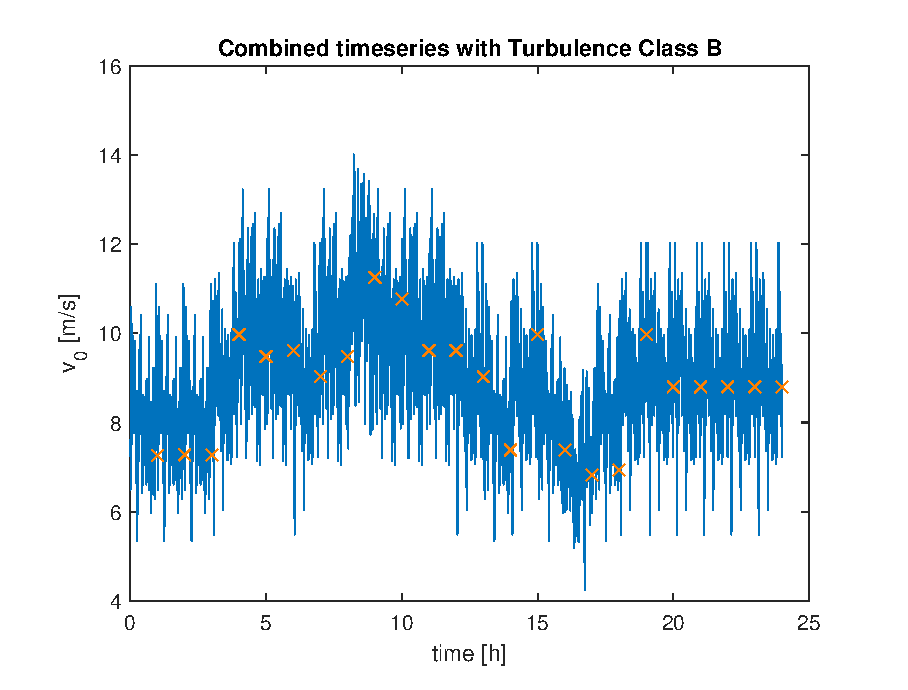
\includegraphics[width=12cm]{Figures/TurbWindField.eps}
	\caption{Combined time series with turbulence class B}
	\label{fig:TurbWindField}
\end{figure}    
